\section{Interatomic Potentials}

\subsection{Introduction}

An interatomic potentials, as used in this work and Molecular Dynamics computer codes, is a function or a set of functions that describe the energy and force between atoms.  Simpler functions represent the potential energy between pairs of atoms only, but more complicated functions have been used in molecular dynamics since the 1980s that also attempt to represent the many body nature of materials, which applies in particular to metals.


\subsection{Pair Potentials}

A pair potential only considers pairs of nearby atoms, one pair at a time, and does not consider the effect of any other nearby atoms.  Where an alloy is being modelled, there will be a pair potential function for each element and element combination; 1 for a single element, 3 for a two element alloy, 6 for a three element alloy and so on.


\FloatBarrier
\subsubsection{Lennard-Jones}

The Lennard-Jones potential was proposed in the 1920s and has both an attractive term and a repulsive term; the $(r_m/r)^12$ becomes much larger than the $(r_m/r)^6$ term at close distances, and this mimics the coulomb repulsion as two atoms are pushed closer together.  At larger seperations, the attractive term dominates.

\begin{equation}
\begin{split}
V(r) = e \left(\left(\frac{r_m}{r}\right)^12 - 2 \left(\frac{r_m}{r}\right)^6\right)
\end{split}
\label{eq:eqLennardJones}
\end{equation}

\begin{figure}[!htbp]
  \begin{center}
    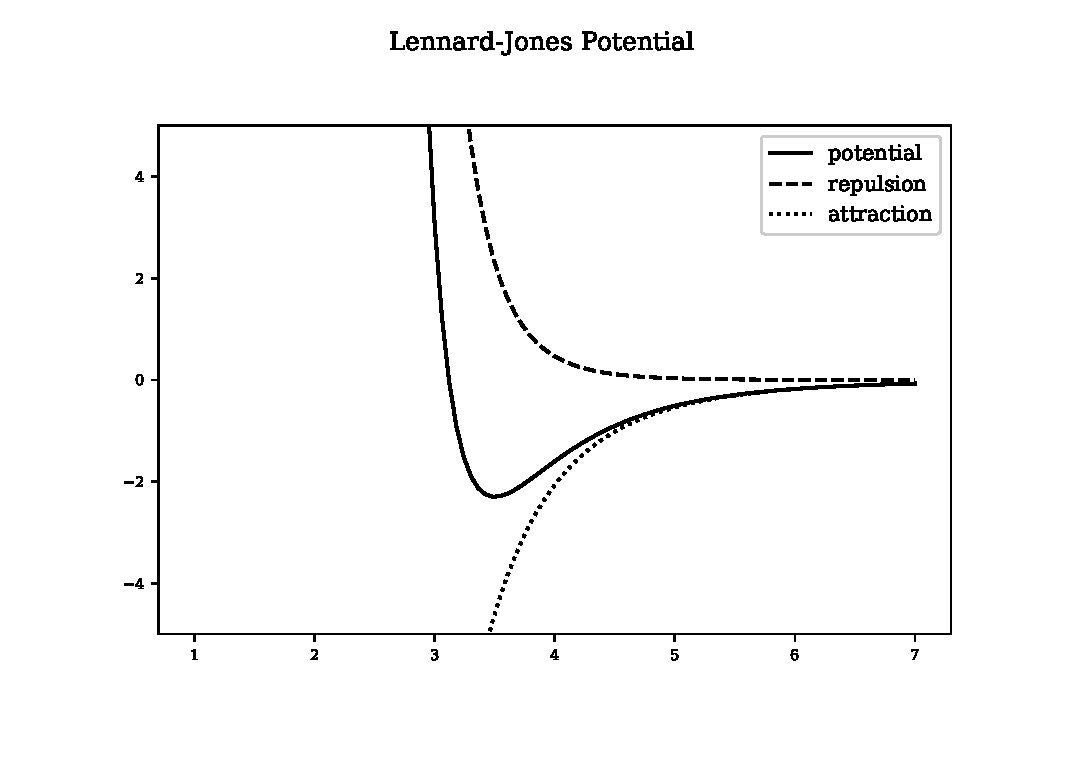
\includegraphics[scale=0.70]{chapters/background_potential_fitting/plots/lennard_jones.eps}[scale=0.6]
    \caption{Graph caption}
    \label{graph:graph1}
  \end{center}
\end{figure}



\FloatBarrier
\subsubsection{Morse Potential}

The Morse potential was proposed five years after the Lennard-Jones potential.  It also has an attractive and repulsive term, but it uses the exponential function rather than 6th and 12th powers.

\begin{equation}
\begin{split}
V(r) = exp(-2 a (r - re)) - 2 exp (-a*(r - re))
\end{split}
\label{eq:eqLennardJones}
\end{equation}

\begin{figure}[!htbp]
  \begin{center}
    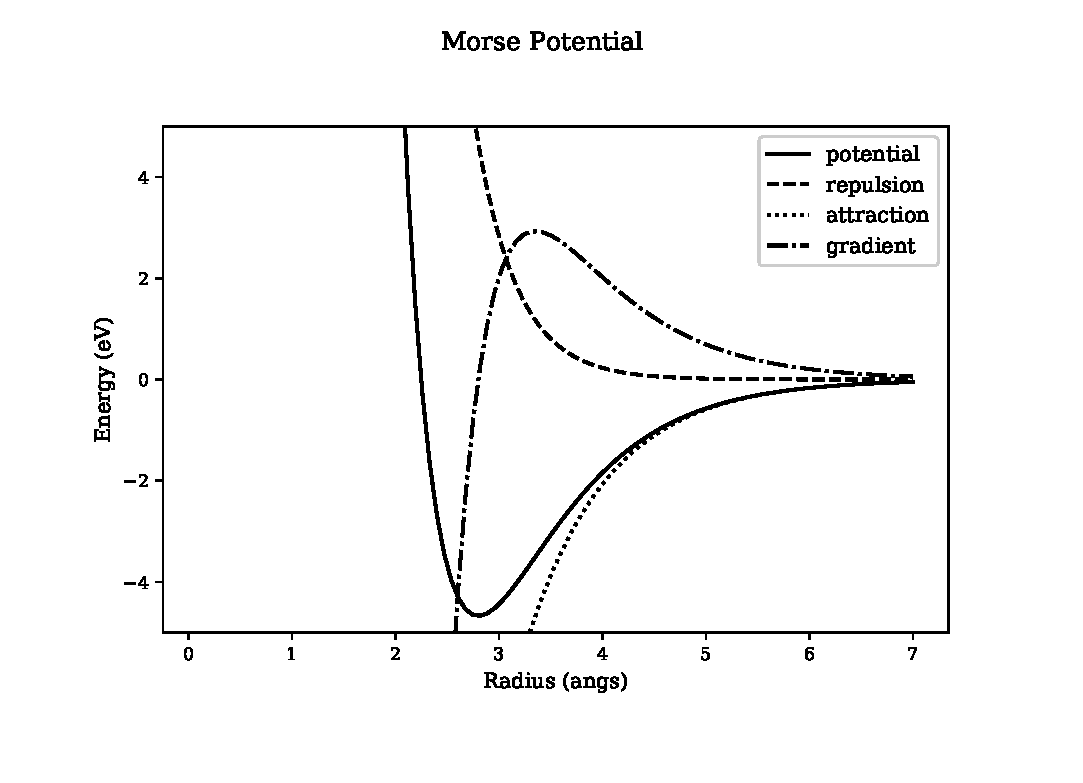
\includegraphics[scale=0.70]{chapters/background_potential_fitting/plots/morse.eps}[scale=0.6]
    \caption{Graph caption}
    \label{graph:graph1}
  \end{center}
\end{figure}



\FloatBarrier
\subsubsection{Buckingham Potential}


\begin{equation}
\begin{split}
V(r) = A * exp(-B * r) - \frac{C}{r**6}
\end{split}
\label{eq:eqLennardJones}
\end{equation}

\begin{figure}[!htbp]
  \begin{center}
    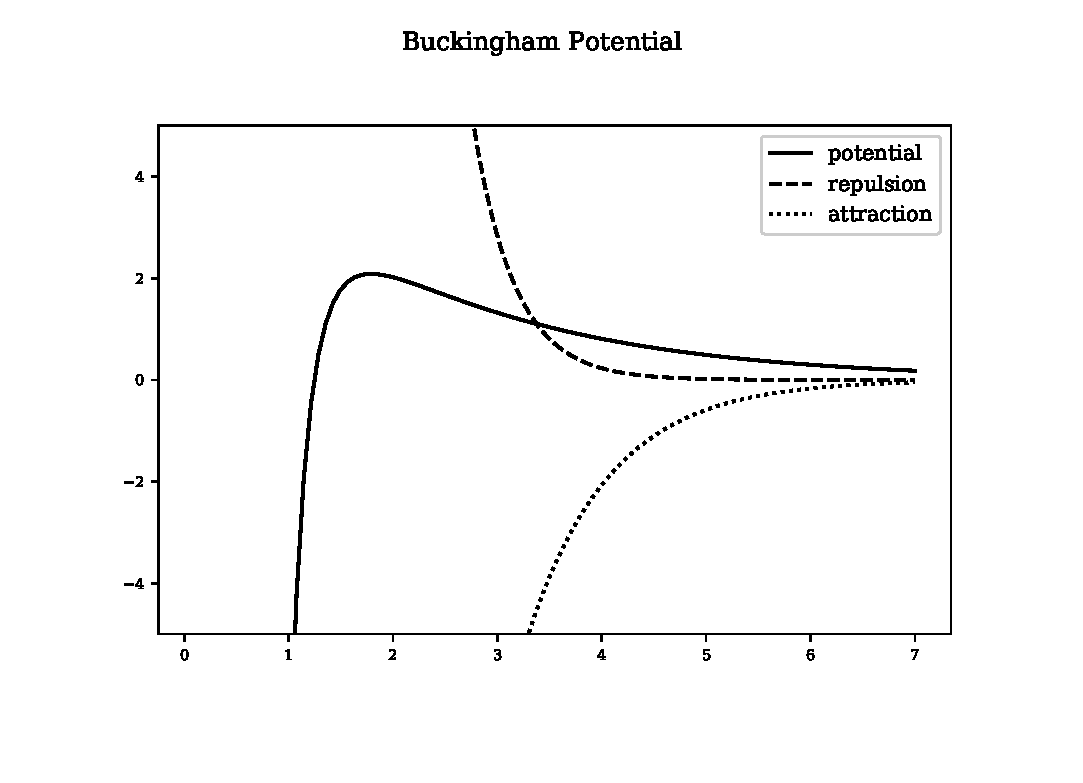
\includegraphics[scale=0.70]{chapters/background_potential_fitting/plots/buckingham.eps}[scale=0.6]
    \caption{Graph caption}
    \label{graph:graph1}
  \end{center}
\end{figure}


\FloatBarrier
\subsubsection{ZBL Universal Potential Function}

It became clear, while experimenting with a number of existing potentials and molecular dynamics programs, that at the very least modifications to those potentials would need to be made for small atom seperations.  A simulation to model a projectile failed early on due to the projectile's proximity to target atoms, resulting in the MD code returning an error as the seperation was out of the range of the potential.

The Ziegler Biersack Littmark (ZBL) potential, between an atom of charge $Z_i$ and $Z_j$ is set out in the SRIM manual\cite{srimbook}.


\begin{equation}
\begin{split}
V_{zbl}(r_ij, Z_i, Z_j) = \frac{1}{4 \pi \epsilon_0} \frac{Z_i Z_j}{r_{ij}} \phi \left( \frac{r_{ij}}{a_{ij}} \right) \\
\text{where } \epsilon_0 = 8.85419\times 10^{-12} 
\end{split}
\label{eq:eqLennardJones}
\end{equation}

The parameters of the Universal screening potential function are as follows:

\begin{equation}
\begin{split}
\phi(x) = 0.181 e^{-3.2x} + 0.5099 e^{-0.9423x} + 0.2802 e^{-0.4029x} + 0.02817 e^{-0.2016x} \\
\text{where } a_{ij} = \frac{0.8854 a_0}{Z^{0.23}_i + Z^{0.23}_j} \\
\text{and } a_0 = 0.529 \text{angstrom}
\end{split}
\label{eq:screeningPotential}
\end{equation}


\begin{figure}[!htbp]
  \begin{center}
    \includegraphics[scale=0.70]{chapters/background_potential_fitting/plots/zbl.eps}[scale=0.6]
    \caption{Graph caption}
    \label{graph:graph1}
  \end{center}
\end{figure}





\subsection{Many Body Potentials}

This work is focused on metals, and two popular, and closely related potentials, will be discussed in this section.

\subsubsection{Finnis-Sinclair}

The Finnis-Sinclair potential was published in 1984 and it introduced both a pair potential and an embedded term to take into account the cohesive energy dependent on the local electron density.  The pair term represents the repulsion between the atoms whereas the embedding functional glues the atoms together in the solid.  

The tight-binding that this potential is based on is represented by the functional: square root of the density.  The potential for a single element model consists of a pair function, a density funstion and a tight-binding functional.

\begin{equation}
\begin{split}
u^{A,A} = \sum_{i \ne j}^{N}(r) v^{A,A}(r_{i,j}) \newline
rho^{A}_{i}(r) = \sum_{j, j \ne i}^{N} \phi(r_{ij}) \newline
F^{A} = \sum_{i}^{N}
\end{split}
\label{eq:eqFinnisSinclair}
\end{equation}


\subsubsection{Embedded Atom Method}

The Embedded atom method was also developed in the 1980s.  It was developed with metals in mind, and in many ways is a more flexible variant of the Finnis-Sinclair potential.  It too has a pair and density function, but the functional of the EAM potential is not restricted to a square root.


\begin{equation}
\begin{split}
U_{EAM} = \frac{1}{2} \sum \limits_{i=1}^{N} \sum \limits_{j\ne i}^{N} V_{ij}(r_{ij}) + \sum \limits_{i=1}^{N} F[\rho _{i}] \\
\textnormal{where   } \rho_{i} = \sum \limits_{j=i,j \ne i}^{N} \rho_{ij}(r_{ij})
\end{split}
\label{eq:eqEAM}
\end{equation}


\subsection{Two Band Embedded Atom Method}

There are several variations of the EAM potential, and one of particular interest to us is the two-band model EAM (2BMEAM) that has two electron density and embedding energy terms.  This formalism was originally developed to model Caesium\cite{twobandackland}, and the transition of electrons between S and D bands under pressure, but it has been modified to apply to alloys.

An alloy version of the two-band model was developed by Olsson et al. to investigate the α-prime phase formation in Fe-Cr (15).  It was further developed by Bonny et al to provide a reliable EAM type potential to model high-chromium ferritic alloys (16).  This potential correctly predicts the change of sign in mixing enthalpy as the local concentration of Chromium changes, and the functions take the following form.

\begin{equation}
\begin{split}
U_{EAM} = \frac{1}{2} \sum \limits_{i=1}^{N} \sum \limits_{j\ne i}^{N} V_{ij}(r_{ij}) + \sum \limits_{i=1}^{N} F_{D}[\rho _{d,i}] + \sum \limits_{i=1}^{N} F_{S}[\rho _{s,i}] \\
\textnormal{where   } \rho_{d,i} = \sum \limits_{j=i,j \ne i}^{N} \rho_{d,ij}(r_{ij})
\textnormal{  and  } \rho_{s,i} = \sum \limits_{j=i,j \ne i}^{N} \rho_{s,ij}(r_{ij})
\end{split}
\end{equation}

This allows a second embedding functional and electron density function to add/subtract energy to an atom when mixed as an alloy, but reverts to the original EAM for that element when in local concentrations of like-atoms.







\subsection{Many Bands for the Embedded Atom Method}

\begin{equation}
\begin{split}
U_{EAM} = V_{pair} + \sum_{b}^B F_b (\rho_b)
\frac{1}{2} \sum \limits_{i=1}^{N} \sum \limits_{j\ne i}^{N} V_{ij}(r_{ij}) + \sum \limits_{b=1}^{B} \sum \limits_{i=1}^{N} F_{b}[\rho _{b,i}] \\
\textnormal{where   } \rho_{b,i} = \sum \limits_{j=i,j \ne i}^{N} \rho_{b,ij}(r_{ij}) \\
\textnormal{and B total number of bands, 1, 2, 3 etc}
\end{split}
\end{equation}


\subsection{Function Types used by EAM and Two-Band EAM}

In previous work, their are a wide range of functions used to represent the pair potential, density and embedding functional.  These range from those that preserve and attempt to replicate the physics, to those that do away with knowledge of the physics underlying the potentials altogether.  The pair potentials already covered here may also be used as the pair function component of the EAM or Two-Band EAM potentials.

A full list of the functions considered and included in the potential fitting code that resulted from this work is included in the appendix.  Only polynomial splines will be discussed further here.



\subsubsection{Polynomial Splines}

The form of polynomial spline used in the literature is a sum of N cubic polynomials that, by way of the Heaviside step function and their form, cutoff neatly at the desired radius.  The cutoff radii are fixed and, during the fit of a potential, just the coefficients of each cubic spline are varied.

\begin{equation}
\begin{split}
V(r) = \sum_i^N a_i (r - r_i)^3 H(r_i - r) \\
\text{where } \\
H(x) = \left\{ \begin{matrix} 0 & x<0 \\  1 & x >= 0 \end{matrix} \right . 
\end{split}
\label{eq:cubicSpline}
\end{equation}


\subsubsection{Polynomial Knot to Knot Splines}

So far, analytic potentials have been discussed.  There are existing potentials that do not have an analytic form, but are tabulated data that have the properties that they are continuous and have a continuous first derivatives.  In attempting to fit or re-fit tabulated data, it would be problematic to adjust each data point individually given the number of data points and the requirement to have a continuous well behaved function with continuous first derivatives.

\begin{figure}[h]
  \begin{center}
    \includegraphics[scale=0.70]{chapters/background_potential_fitting/plots/spline.eps}[scale=0.6]
    \caption{Graph caption}
    \label{graph:graph1}
  \end{center}
\end{figure}

The tabulated function is divided into sections, and the start and end of each section forms the knot of the spline.  A polynomial may be splined between these knots, but the order of polynomial will depend on the data available.  Immediately, the x and y positions are known: $x_a, x_b, f(x_a), f(x_b)$.  A first order polynomial has two unknowns, and so these unknowns may be calculated using linear algebra.

\begin{equation}
\begin{split}
c_0 + c_1 x_a = y_a \\
c_0 + c_1 x_b = y_b \\
\end{split}
\label{eq:cubicSpline}
\end{equation}

One of the requirements for the potential is to have a continuous first derivative, and this requires knowledge of the first derivative at each knot.  In the figure, the knots are shown as circles.  By taking several points near to each knot, shown as squares, the derivative at each knot may be calculated by interpolation.  This allows a third order polynomial to be used:


\begin{equation}
\begin{split}
      P_{1} = \left( x_A, f(x_A) \right) \\
      P_{2} = \left( x_A, f'(x_A) \right) \\
      P_{3} = \left( x_B, f(x_B) \right) \\
      P_{4} = \left( x_B, f'(x_B) \right)
\end{split}
\label{eq:eqSplineThreePoints}
\end{equation}

\begin{equation}
\begin{split}
c_0 + c_1 x_a + c_2 x_a^2 + c_3 x_a^3 = y_a \\
0 + c_1 + 2 c_2 x_a + 3 c_3 x_a^2 = y_a' \\
c_0 + c_1 x_b + c_2 x_b^2 + c_3 x_b^3 = y_b \\
0 + c_1 + 2 c_2 x_b + 3 c_3 x_b^2 = y_b' \\
\end{split}
\label{eq:cubicSpline}
\end{equation}

Rewriting as matrices:

\begin{equation}
\begin{split}
      \begin{bmatrix}
      1  &  x_a  &  {x_a}^2  &  {x_a}^3     \\
      0  &  1    &  2 x_a    &  3 {x_a}^2   \\
      1  &  x_b  &  {x_b}^2  &  {x_b}^3     \\
      0  &  1    &  2 x_b    &  3 {x_b}^2
      \end{bmatrix}
      \begin{bmatrix}
      c_0 \\
      c_1 \\ 
      c_2 \\ 
      c_3
      \end{bmatrix}
      = 
      \begin{bmatrix}
      f(x_a) \\
      f'(x_a) \\ 
      f(x_b) \\ 
      f'(x_b)
      \end{bmatrix}
\end{split}
\label{eq:eqSplineThreeMatrix}
\end{equation}

By interpolating and calculating the second order derivative at each knot, a 5th order polynomial may also be splined between pairs of knots.  This approach may be modified to spline functions of the form $exp(p(r))$ between knots, and this is useful for splining between a ZBL or similar repulsive function at small r and a function of a different form at larger r.


\begin{equation}
\begin{split}
\text{where } \\
V(r) = \left\{ \begin{matrix} 
ZBL(r, q_1, q_2) & r<= r_a \\  
exp(a+br+cr^2 + dr^3) & r_a < r < r_b \\ 
v(r) & r_b < r < r_{cut} \\ 
0 & r >= r_{cut} \\
\end{matrix} \right . 
\end{split}
\label{eq:cubicSpline}
\end{equation}





\subsubsection{Tending to Zero at the Cutoff Radius}

It is desireable for the functions to be well behaved and continuous.  The coulomb force between two charged particles reduces smoothly until theoretically at an infinite separation; it doesn't reach a set separation and abruptly drops to zero.  It is impossible and unhelpful to consider an infinite separation which is why the cutoff radius has been introduced.  It represents the seperation where the potential has reachead zero; at the very least it's a tradeoff between accuracy and the computing time available for the problem.

The pair potential should therefore drop off to 0 at the cutoff radius, and be equal to zero for larger separations.  The electron density spherically around an atom should also smoothly drop off to zero, and similarily it should be equal to zero for distances larger than the cutoff.  The embedding energy is dependent on the density at the location of the atom embedded.  The embedding function will not necessarily drop off to zero, and it depends on the density and not the separation.

In a molecular dynamics simulation, the neighbour list will usually be built considering atoms slightly more separated than the cutoff radius of the functions.  This allows the same neighbour list to be used for several time steps, before the need to update.  








\subsection{Calculating Energy, Force and Stress}

Molecular dynamics simulations do not need to include the weak or strong force, and the gravitational force between atoms in the simulated material are so weak in comparison the the electromagnetic force, they can also be ignored.  There is a force between all the atoms within a real material, but the electromagnetic force is inversely proportionally to the seperation of the atoms.  Above a certain separation, the electromagnetic force can also be ignored, in order to simplify the computation.

\subsubsection{Neighbour List}

A cutoff radius can be introduced to limit the number of neighbours.  As the lattice parameter decreases, the atoms are brought closer together, and as the cutoff radius is increased more atoms are considered to be within the sphere of influence of one another.  Both increase the number of neighbours each atom has.

\begin{figure}[!htbp]
  \begin{center}
    \includegraphics[scale=0.40]{chapters/background_potential_fitting/plots/atom_neighbours.eps}
    \caption{Graph caption}
    \label{graph:graph1}
  \end{center}
\end{figure}

Building a neighbourlist may take a long while, depending on the parameters.  If a simplistic approach is taken, for N atoms in the supercell, there will be $27N^2$ checks between atoms to see whether they are within the cutoff radius of one another.  For larger numbers of atoms in a supercell, the whole may may be decomposed into smaller domains.

For example, a 16x16x16 FCC supercell, containing 16,384 atoms, would require looping $27 \times 16,384^2 = 7.25 \times 10^9$ times.  Breaking the supercell into 64 smaller domains with 256 atoms in each, reducing the problem to $64 \times 27 \times 256^2 = 1.13 \times 10^8$ loops.

For this work, the supercells used to calculate bulk properties from the interatomic potentials, and the configurations generated by DFT, contain fewer than 1,000 atoms, removing the need to decompose the configuration into smaller subcells.

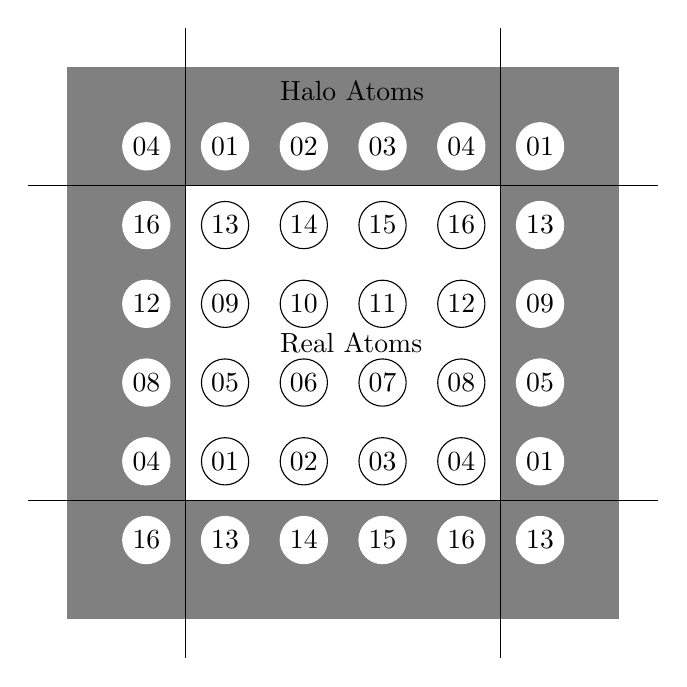
\begin{tikzpicture}
\filldraw [gray] (0.5,0.5) -- (0.5,7.5) -- (7.5,7.5) -- (7.5,0.5) -- (0.5,0.5);
\filldraw [white] (2.0,2.0) -- (2.0,6.0) -- (6.0,6.0) -- (6.0,2.0) -- (2.0,2.0);
\draw (0,2) -- (8,2);
\draw (0,6) -- (8,6);
\draw (2,0) -- (2,8);
\draw (6,0) -- (6,8);
\draw (2.5,2.5) circle [radius=0.3] node {$01$};
\draw (3.5,2.5) circle [radius=0.3] node {$02$};
\draw (4.5,2.5) circle [radius=0.3] node {$03$};
\draw (5.5,2.5) circle [radius=0.3] node {$04$};
\draw (2.5,3.5) circle [radius=0.3] node {$05$};
\draw (3.5,3.5) circle [radius=0.3] node {$06$};
\draw (4.5,3.5) circle [radius=0.3] node {$07$};
\draw (5.5,3.5) circle [radius=0.3] node {$08$};
\draw (2.5,4.5) circle [radius=0.3] node {$09$};
\draw (3.5,4.5) circle [radius=0.3] node {$10$};
\draw (4.5,4.5) circle [radius=0.3] node {$11$};
\draw (5.5,4.5) circle [radius=0.3] node {$12$};
\draw (2.5,5.5) circle [radius=0.3] node {$13$};
\draw (3.5,5.5) circle [radius=0.3] node {$14$};
\draw (4.5,5.5) circle [radius=0.3] node {$15$};
\draw (5.5,5.5) circle [radius=0.3] node {$16$};
\filldraw [white] (1.5,1.5) circle [radius=0.3] node [text=black] {$16$};
\filldraw [white] (1.5,2.5) circle [radius=0.3] node [text=black] {$04$};
\filldraw [white] (1.5,3.5) circle [radius=0.3] node [text=black] {$08$};
\filldraw [white] (1.5,4.5) circle [radius=0.3] node [text=black] {$12$};
\filldraw [white] (1.5,5.5) circle [radius=0.3] node [text=black] {$16$};
\filldraw [white] (1.5,6.5) circle [radius=0.3] node [text=black] {$04$};
\filldraw [white] (2.5,6.5) circle [radius=0.3] node [text=black] {$01$};
\filldraw [white] (3.5,6.5) circle [radius=0.3] node [text=black] {$02$};
\filldraw [white] (4.5,6.5) circle [radius=0.3] node [text=black] {$03$};
\filldraw [white] (5.5,6.5) circle [radius=0.3] node [text=black] {$04$};
\filldraw [white] (6.5,6.5) circle [radius=0.3] node [text=black] {$01$};
\filldraw [white] (6.5,2.5) circle [radius=0.3] node [text=black] {$01$};
\filldraw [white] (6.5,3.5) circle [radius=0.3] node [text=black] {$05$};
\filldraw [white] (6.5,4.5) circle [radius=0.3] node [text=black] {$09$};
\filldraw [white] (6.5,5.5) circle [radius=0.3] node [text=black] {$13$};
\filldraw [white] (6.5,1.5) circle [radius=0.3] node [text=black] {$13$};
\filldraw [white] (2.5,1.5) circle [radius=0.3] node [text=black] {$13$};
\filldraw [white] (3.5,1.5) circle [radius=0.3] node [text=black] {$14$};
\filldraw [white] (4.5,1.5) circle [radius=0.3] node [text=black] {$15$};
\filldraw [white] (5.5,1.5) circle [radius=0.3] node [text=black] {$16$};
\node[text width=3cm] at (4.7,7.2) {Halo Atoms};
\node[text width=3cm] at (4.7,4.0) {Real Atoms};
\end{tikzpicture}



To build the neighbour list a halo configuration is created such that it lies on top of the real atoms, but extends at least as far as the cut off radius on each side of the real simulation box.  Periodic boundary conditions are used to construct the halo.

Once the halo list is computed, the neighbour list may also be computed by looping through the real atoms and halo atoms.  A simple pseudo coded sub routine is given below.


\begin{lstlisting}[style=sPseudo,caption={Simple genetic optimisation subroutine}]

// real_atoms - array holding coordinates of all real atoms
// halo_atoms - array holding coordinates of all halo atoms
// real_ids - unique id for each atom
// halo_ids - unique atom ids for halo atoms
// nlist_ids - array to store ids
// nlist_r - array to store separation

// Define the cutoff and counter start value
r_cut = 5.0
nl_counter = 1

// Calculate square
r_cut_sq = r_cut ** 2

// Loop over all real atoms
DO n_real = 1, real_atom_count
  // Loop over all halo atoms
  DO n_halo = 1, halo_atom_count
    IF (real_ids(n_real) .LT. halo_ids(n_halo)) THEN
      r(1:3) = halo_atoms(n_halo, :) - real_atoms(n_real, :)
      r_sq = SUM(r(1:3) * r(1:3))
      IF (r_sq .LE. r_cut_sq) THEN          
        r_mag = sqrt(r_sq)          
        nlist_ids(nl_counter, 1) = real_ids(n_real)
        nlist_ids(nl_counter, 2) = halo_ids(n_halo)        
        nlist_r(nl_counter, 1) = r_mag
        nlist_r(nl_counter, 2:4) = r(1:3)/r_mag
        nl_counter = nl_counter + 1
      END IF
    END IF
  END DO
END DO 
\end{lstlisting}

The resulting list will contain unique a pair combinations; i.e. the pair atom 1 and atom 2 will only be recorded once, and not also as atom 2 and atom 1.


\subsubsection{Computing Total Energy}

The total energy of the system is the sum of the individual energies for the atoms in the simulation.  The type of atom (or pairs of atoms) will determine which function is used.

First, to compute the pair potentials:

\begin{itemize}
\item set the total energy of the system equal to zero
\item set the starting energy for each atom in the system to zero
\item loop through the atom pairs in the entire neighbour list
\item for each atom pair, A and B, use the known separation and the potential function to compute the potential energy on atom A due to B and vice versa
\item add this potential energy to both A and B
\item after looping through the neighbour list, add all the energies due to the pair potential to the total energy
\end{itemize}

For an EAM or 2BEAM potential, the densities and embedding energies must also be computed:

\begin{itemize}
\item set the electron density at the position of (for each) atom to zero
\item loop through the atom pairs in the entire neighbour list
\item for each atom pair, using the density function for the atom A, the density at atom B due to atom A will be calculated and added to the density at atom B
\item if the atoms are both of the same type the same density will be added to atom A due to atom B
\item if the atom types are different, using the density function for the atom B, the density at atom A due to atom B will be calculated and added to the density at atom A
\item following looping through the neighbour list, to calculate the densities at each atom, the list of atoms will be looped through
\item for each atom, the density value at the position of that atom, will be input into the appropriate embedding function to calculate the embedding portion of the energy
\item add all the embedding energies to the total energy of the system
\end{itemize}

For a 2BEAM potential, repeat the above procedure for the second group of density functions and embedding functions (do not repeat calculation of the pair potentials).


\subsubsection{Computing Forces on Atoms}

In order to calculate the forces on the atoms with an EAM or 2 Band EAM potential, the neighbour list and atom list will need to be looped through several times.  First, the pair potential and force due to the pair potential must be calculated by a complete loop through the neighbour list.  At the same time, the density at each atom location is also calculated.  The embedding energy may then be computed by looping through all the atoms and using the electron density at each atom to give the energy of the atom embedded in that density.  The third and final loop will run through the neighbour pairs in the neighbour list once more computing the force on each atom due to it's embedding.

The force on each atom, due to surrounding atoms, may be split into two; force due to the pair potential, and the force due to the embedding of the atom\cite{dlpolymanual}.

\begin{equation}
\begin{split}
F^k_{pair} = -\sum \limits_{j=1, j \ne k}^{N} \frac{\partial V_{kj} (r_{kj}}{\partial r_{kj}} \frac{\vec{r}_{kj}}{\lvert\vec{r}_{kj}\lvert} \\
F^k_{embed} = -\sum \limits_{j=1, j \ne k}^{N} \left(\frac{\partial F}{\partial \rho_k} + \frac{\partial F}{\partial \rho_j} \right) \frac{\partial \rho (r_{kj})}{\partial r_{kj}} \frac{\vec{r_{kj}}}{r_{kj}}
\end{split}
\label{eq:eqLennardJones}
\end{equation}


\subsubsection{Computing Stress}

The stress is be calculated assuming the system is at 0K\cite{wikivirialstress}.

\begin{equation}
\begin{split}
\tau_{ij} = \frac{1}{2 V} \sum_{k,l \in V} \left({x_i}^{(l)} - {x_i}^{(k)} \right) {f_j}^{(kl)}
\end{split}
\label{eq:eqVirialStress}
\end{equation}

Within the computer code, the individual force components between pairs of atoms are stored as well as an equal sized array of vectors representing their spatial separation.  Those pairs with one atom in the halo around the simulation box are used to calculate the stress on the simulation box.


\subsubsection{Pseudo Code for the Energy, Force and Stress Subroutine}

\begin{lstlisting}[style=sPseudo,caption={Pseudo Code for Energy and Stress Force Calculation}]

electron_density[1:n_atoms, 1:bands] = 0.0  // electron density at each atom
density_grad_ab[:,:] = 0.0                  // grad density function
density_grad_ba[:,:] = 0.0                  // grad density function
energy = 0.0                                // total energy
forces[:,:] = 0.0                           // forces each atom, 3D
force_between_pairs[:,:] = 0.0              // used to store force between pairs, for stress computation
stress[:,:] = 0.0D0

// LOOP 1 - Pair energy, force and calculate densities
DO n = 1, neighbour_count
  E = get_PairEnergy(atom_a, atom_b, r[n,:])
  F[:] = get_PairForce(atom_a, atom_b, r[n,:])

  // Save energy
  energy = energy + E

  // Save Force
  f[atom_a, :] = f[atom_a, :] - F[:]
  f[atom_b, :] = f[atom_b, :] + F[:]
  force_between_pairs[:,:] = force_between_pairs[:,:] - F[:]   // Used to calculate stress
  
  // Loop through density bands
  DO band = 1, bands
    // Electron density at A due to atom B
    electron_density[atom_a, b] = get_Density(atom_b, r)
    density_grad_ab[n, band] = get_DensityGradient(atom_b, r)
  
    // Electron density at B due to atom A
    electron_density[atom_a, band] = get_Density(atom_a, r)
    density_grad_ba[n, band] = get_DensityGradient(atom_a, r)
  END DO
END DO

// LOOP 2 - Embedding energy
DO n = 1, atom_count
  // Loop through density bands
  DO band = 1, bands
    energy = energy + get_EmbeddingEnergy(n, band)
  END DO
END DO

// LOOP 3 - Embedding force
DO n = 1, neighbour_count
  // Loop through density bands
  DO band = 1, bands
    epA = get_EmbeddingGradient(atom_a, electron_density(atom_a, b))
    epB = get_EmbeddingGradient(atom_b, electron_density(atom_b, b))

    F[:] = (epA * density_grad_ba(n, band) + epB * density_grad_ab(n, band)) * r[n, :]

    f[atom_a, :) = f(atom_a, :) - F[:] 
    f(atom_a, :) = f(atom_a, :) + F[:] 
    
    force_between_pairs[:,:] = force_between_pairs[:,:] - F[:]   // Used to calculate stress
  END DO
END DO

// LOOP 4 STRESS
DO n = 1, neighbour_count
  // Only compute if the second atom is in the halo 
  IF(nlisthalo(n))THEN  
    DO i = 1,3
      DO j = 1,3
        stress[i,j] = stress[i,j] + (r[n, i] * force_between_pairs[n,j])
      END DO
    END DO
  END IF
END DO
stress[1:3, 1:3] = stress[1:3, 1:3] / (2.0 * volume)

\end{lstlisting}



\subsection{Choice of Functions and Functionals}

The EAM potential, for n elements, is made up of n pair functions, $n(n+1)/2$ density functions and $n(n+1)/2$ embedding functionals.  The choice of function varies greatly.  Irrespective of the choice of function, there are a number of desireable properties:


\begin{itemize}
\item the function should be well behaved
\item this should be true for the derivative and second derivative - ideally, these should be continuous too
\item the pair and density functions should have a cutoff, and the value at this cutoff should be zero
\end{itemize}

\subsubsection{ZBL to Pair Function Spline}

Certain functions may behave oddly at small values of atom seperation, and this can be seen for the Buckingham potential, where the potential may drop sharply to negative values, pulling the modelled atoms together.  The ZBL function is a good choice to model higher energy atoms that do come close together.  It may be desireable to keep the characteristics for the 








\subsubsection{A One Time Neighbour List}

As there are only static calculations in this work, the neighbour list will only need to be computed once.  The potential functions will change during the fitting process, but the configuration, and neighbourlist, is frozen in place from the start to the end of the fitting procedure.





\subsection{Sacrificing Physical Elegance}

There doesn't exist a generic formula that describes the energy and forces between atoms.  Even first priciples calculations rely of approximations, and the knowledge of an exact exchange functional eludes us.  While it would be satisfying to derive a potential that reflects the fundamental physics, it may be something that is forever out of our reach.

It is more useful to develop a potential that replicates the behavior of DFT calculations (matches the forces, energies, stresses etc) and reproduces material properties such as its elastic constants.  If it can do this, and give insights into the material in a way that is not yet possible experimentally, does it matter if the physical elegance is lost?








